% =========================================================================
\section{Preliminaries}
\label{section:preliminaries}
% =========================================================================


 
% =========================================================================
\subsection{CSP and Refinement}

% =========================================================================

\subsubsection*{Communicating Sequential Processes} @todo
\fxwarning{alcc: I can make this small contribution.}


Throughout this paper, the alphabet of CSP processes $P$ is denoted by $\Sigma$. 
Since we are only considering ``classical'' CSP processes, the alphabet is always finite.

% =========================================================================
\subsubsection*{Normalised Transition Graphs for CSP Processes}
\label{sec:ntg}

As shown in~\cite{Roscoe:1994:CME:197600}, any finite-state CSP process $P$
can be represented by a \emph{normalised transition graph}
$$
G(P) = ( N, \ii n, \Sigma, t : N\times\Sigma \pfun N, r : N \fun \mathbb{P}\mathbb{P}(\Sigma)),
$$
with nodes $N$, initial node $\ii n\in N$, and process alphabet $\Sigma$. The
partial \emph{transition function} $t$ maps a node $n$ and an event
$e\in\Sigma$ to its successor node $t(n,e)$, if, and only if, $(n,e)$ is in
the domain of $t$, that is, there is a transition from $n$ with label $e$.
Normalisation of $G(P)$ is reflected by the fact that $t$ is a function.

A finite sequence of events $s\in\Sigma^*$ is a \emph{trace} of $P$, if there
is a path through $G(P)$ starting  at $\ii n$ whose edge labels coincide with
$s$. The set of traces of $P$ is denoted by $\trc(P)$. If $s\in\trc(P)$, then
the process corresponding to $P$ after having executed $s$ is denoted by
$P/s$. Since $G(P)$ is normalised, there is a unique node reached by applying
the events from $s$ one by one, starting in $\ii n$. Therefore, $G(P)/s$  is
also well defined.

By $[n]^0$ we denote the \emph{initials} of $n$:~the set of events occurring
as labels in any outgoing transitions.
$$
[n]^0 = \{ e\in\Sigma~|~(n,e)\in\dom~t \}
$$
We also use this notation for CSP processes:~$[P]^0$ is the set
of events $P$ may engage into, in other words, the initials of $P$ after the
empty trace of events, that is, $initials(P/\langle\rangle)$ as defined
in~\cite{Roscoe2010}.

The total function $r$ maps each node $n$ to its \emph{refulsals} $r(n) =
\refs(n)$. Each element of $r(n)$ is a set of events that the CSP process $P$
might refuse to engage into, when in a process state corresponding to $n$.
The number of refusal sets in $\refs(P/s)$ specifies the degree of
nondeterminism that is present in process state $P/s$: the more refusal sets
contained in  $\refs(P/s)$, the more nondeterministic is the behaviour in
state $P/s$. If $P/s$ is deterministic, its refusals coincide with the set of
subsets of $\Sigma - [P/s]^0$, including the empty set.

For finite CSP processes, since the refusals of each process state are
subset-closed~\cite{Hoare:1985:CSP:3921,Roscoe2010}, $\refs(P/s)$ can be
re-constructed by knowing the set of \emph{maximal refusals}
$\maxrefs(P/s)\subseteq\refs(P/s)$. More formally, the maximal refusals
$\maxrefs(P/s)$ are defined as
\begin{equation}
\maxrefs(P/s) = \{ R \in\refs(P/s)~|~\forall R'\in \refs(P/s) - \{ R\}: R \not\subseteq R'\}
\end{equation}
Conversely, with the maximal refusals at hand, we can reconstruct the refusals by subset-closure:
\begin{equation}
\refs(P/s) = \{ R'\in\power(\Sigma)~|~\exists R\in \maxrefs(P/s): R'\subseteq R \}.
\end{equation}
To see that this approach works only for finite CSP processes, consider the
example where $\Sigma$ is infinite. In this case,
$\maxrefs(STOP/\langle\rangle)$ is empty, and so we cannot use this set to
calculate the refusals of $STOP$, that is, $\refs(STOP/\langle\rangle)$ as
defined above. As with refusals, we also use the transition graph-oriented
notation $\maxrefs(n) \subseteq r(n)$ to denote the maximal refusals
associated with graph state $n$: if $n$ is the state reached in the
transition graph by following the edge labels in trace $s$, then $\maxrefs(n)
= \maxrefs(P/s)$.

Well-formed normalised transition graphs must not refuse an event of the
fan-out of a state in {\it every} refusal applicable in this state; more
formally,
\begin{equation}
\label{eq:wellformedg}
\forall n\in N, e\in\Sigma: (n,e)\in\dom~t \Rightarrow
\exists R\in \maxrefs(n): e\not\in R
\end{equation}


By construction, normalised transition graphs reflect the \emph{failures
semantics} of finite-state CSP processes:~the traces $s$ of a process are the
sequences of transition associated with paths through the graph,
starting at $\ii n$. The pairs $(s,R)$ with $s\in\trc(P)$ and $R\in
r(G(P)/s)$ represent the failures $\failure(P)$ of $P$.

When investigating  tests for failures refinement, 
the notion of \emph{acceptances}~\cite{Hennessy:1988:ATP:50497} 
which is dual to refusals will also be useful. An acceptance set of $P/s$ is a subset
of the initials $[P/s]^0$, i.e. a subset of events labelling  outgoing transitions
of $G(P)/s$. If the behaviour of  $P/s$ is deterministic, its only acceptance equals
$[P/s]^0$, because $P/s$ will never refuse any of the events contained in this set. If
$P/s$ is nondeterministic, it will internally choose one of it 
\emph{minimal acceptance sets} $A$ and never refuse any event in $A$, while refusing the
events in $\Sigma-A$. The acceptances of 
 $P/s$ are denoted by $\accs(P/s)$, the minimal acceptances by $\minaccs(P/s)$. 
 They fulfil the following rules.
\begin{eqnarray}
A\in \minaccs(P/s) & \Leftrightarrow & \exists R\in\maxrefs(P/s) \wedge A = \Sigma-R
\label{eq:accref}
\\
\bigcup \{ A~|~A\in \accs(P/s)\} & = & [P/s]^0
\label{eq:accinitials}
\\
 X\in\accs(P/s) &\Leftrightarrow & A\in \minaccs(P/s) \wedge A\subseteq X \subseteq [P/s]^0
 \label{eq:accsubset}
\end{eqnarray} 
Note that (\ref{eq:accref}) can be regarded as a definition of minimal acceptances by means
of maximal refusals. Then (\ref{eq:accinitials}) and (\ref{eq:accsubset}) are consequences
of this definition and  the fact that refusals are subset-closed.

Every node of a transition graph can be labelled with with its minimal acceptances, and this information is equivalent to 
that contained in its maximal refusals.

% .....................................................................................
 \begin{figure}
 %%\hspace*{-40mm}
 \begin{center}
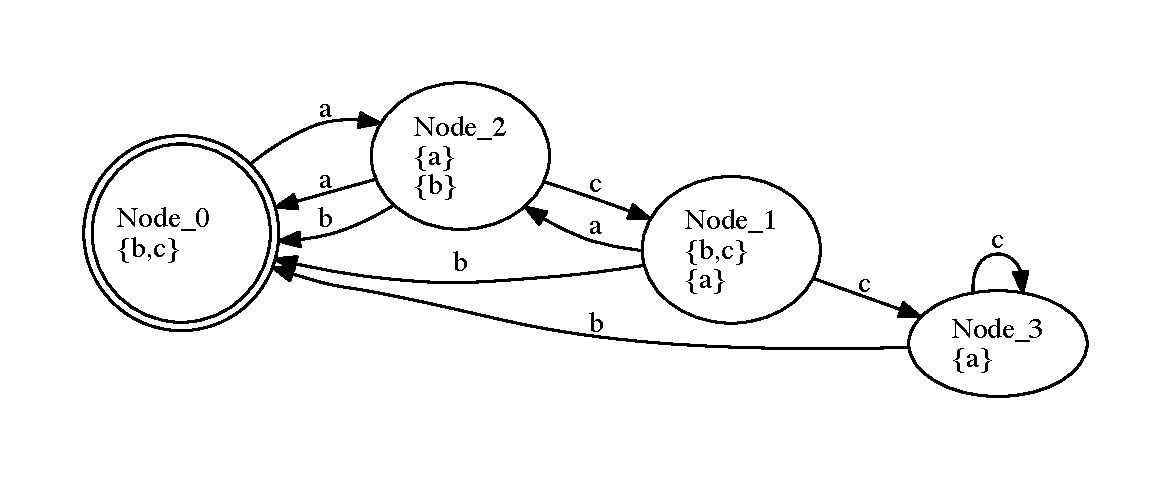
\includegraphics[width=\textwidth]{q0.pdf}
\end{center}
%%\vspace*{-10mm}
\caption{Normalised transition graph of CSP process $P$ from Example~\ref{ex:a}.}
 \label{fig:tga}
 \end{figure}
% .......................................................................................

\begin{example}{ex:a}
Consider the CSP process $P$ defined below, and that the set of events
$\Sigma$ is $\{a,b,c\}$.
\begin{eqnarray*}
P & = & a \then (Q\intchoice R)
\\
Q & = & a \then P \extchoice c \then P
\\
R & = & b \then P \extchoice c \then R
\end{eqnarray*}
Its transition graph $G(P)$ is shown in Fig.~\ref{fig:tga}. Process state
$P/\langle\rangle$ is represented there as Node\_0, with $\{ b,c\}$ as the
only maximal refusal, since $a$ can never be refused, and no other events are
accepted. Having engaged into $a$, the transition emanating from Node\_0
leads to Node\_2 representing  the process state $P/a = Q\intchoice R$. The
internal choice operator induces several refusal sets derived from $Q$ and
$R$. Since these processes accept their initial events in external choice,
$Q\intchoice R$ induces two maximal refusal sets $\{b\}$ and
$\{a\}$. Note that event $c$ can never be refused, since it is not a member
of any maximal refusal.

Having engaged into $c$, the next process state is represented by Node\_1.
Due to normalisation, there is only a single transition satisfying
$t(\text{Node\_2},c) = \text{Node\_1}$. This transition, however, can have
been caused by either $Q$ or $R$ engaging into $c$, so Node\_1 corresponds to
process state $Q/c \intchoice R/c = P \intchoice R$. This is reflected by the
two maximal refusals labelling Node\_1.

Similar considerations explain the other nodes and transitions in
Fig.~\ref{fig:tga}.

Note that the node names are generated by the FDR tool (see next paragraph).
The node numbering is generated by FDR during the normalisation procedure.
Therefore, the node numbers do not reflect the distance from the initial node
Node\_0.
%Node\_2 is a direct successor to the initial node Node\_0, while Node\_1 is a direct successor of Node\_2.
\end{example}

Refinement relations between finite-state CSP processes $P, Q$ 
can be be expressed by means of their normalised transition graphs in the following way.

\begin{lemma}
\label{lemma:tgtrcref}
\begin{eqnarray}
P \lessdet_T Q & \Leftrightarrow & \trc(G(Q)) \subseteq\trc(G(P))
\label{eq:trcrefa}
\\
\label{eq:failrefa}
P \lessdet_F Q & \Leftrightarrow & \trc(G(Q)) \subseteq\trc(G(P)) \wedge {} \nonumber
\\ & & \forall s\in\trc(G(Q)), R_Q\in\maxrefs(G(Q)/s):  \nonumber
\\ & & \tabd
\exists R_P\in\maxrefs(G(P)/s): R_Q\subseteq R_P
\\
\label{eq:failrefb}
P \lessdet_F Q & \Leftrightarrow & \trc(G(Q)) \subseteq\trc(G(P)) \wedge {} \nonumber
\\ & & \forall s\in\trc(G(Q)), A_Q\in\minaccs(G(Q)/s): \nonumber
\\ & & \tabd
\exists A_P\in\minaccs(G(P)/s): A_P\subseteq A_Q
\end{eqnarray}
\end{lemma}

For proving our main theorems, it is necessary to consider the \emph{product} of 
normalised transition graphs. We need this only for the investigation of corresponding traces in reference processes and processes under test. Therefore, the 
labelling of nodes with maximal refusals or minimal acceptances   will be disregard in the 
product construction.
Consider two normalised transition graphs 
\[
G_i = ( N_i, \ii n_i, \Sigma, t_i : N_i\times\Sigma \pfun N_i, r_i : N_i \fun \mathbb{P}\mathbb{P}(\Sigma)),\qquad i = 1,2,
\]
over the same alphabet $\Sigma$. Then their product is defined by
\begin{eqnarray}
G_1\times G_2 & = & (N_1\times N_2,(\ii n_1,\ii n_2), t:(N_1\times N_2)\times\Sigma\pfun (N_1\times N_2))
\\
\dom~t & = & \{ ((n_1,n_2),e)\in (N_1\times N_2)\times\Sigma~|   \nonumber
\\ & & \tabc
(n_1,e)\in\dom~t_1\wedge 
(n_2,e) \in\dom~t_2    \}
\\
t((n_1,n_2),e) & = & (t_1(n_1,e),t_2(n_2,e))\ \text{for $((n_1,n_2),e)\in\dom~t$}
\end{eqnarray}


% =========================================================================

\subsubsection*{Tool Considerations}
The FDR tool~\cite{fdr} supports model checking and semantic analyses of CSP
processes. It provides an API~\cite{fdrmanual} that can be used to construct
normalised transition graphs for CSP processes.

The FDR graph nodes are labelled by \emph{minimal acceptances} instead of
maximal refusals as described above. Since such a minimal acceptance set is
the complement of a maximal refusal, the function $r$ mapping states to their
refusals can be implemented by creating the complements of all minimal
acceptances and then building all subsets of these complements. For practical
applications, the subset closure is never constructed in an explicit way;
instead, sets are checked with respect to containment in a maximal refusal.

@todo

%
%The maximal refusals in each process state $P/s$
% are the complements of
%the minimal acceptances of the node $n$
%corresponding to $P/s$. As a consequences, all failures
%of $P$ are represented by some $(s,R)$, where $s$ is an initialised path through the transition graph and $R\subseteq (\Sigma-A)$ for some minimal acceptance $A\in ac(n)$,
%such that $n$ is the node corresponding to $P/s$.



% =========================================================================
\subsection{Test Cases and Complete Test Suites}
\label{sec:cspcompletedef}
% =========================================================================

@todo




% =========================================================================
\subsection{Minimal Hitting Sets}
\label{sec:hit}
% =========================================================================

When testing for failures refinement, it will become apparent that the main idea of the underlying test strategy can be based on solving a \emph{hitting set problem}. Given a collection of finite sets $C = \{ A_1,\dots,A_n\}$ that are each subsets of a universe $\Sigma$, a \emph{hitting set} $H\subseteq\Sigma$ is a set satisfying
\begin{equation}
\label{eq:hit}
\forall A\in C: H\cap C \neq\varnothing.
\end{equation}

A \emph{minimal hitting set} is a hitting set which cannot be further reduced without losing 
the characteristinc property (\ref{eq:hit}). The problem of determining minimal hitting sets is known to be NP-hard~\cite{Book1975-BOOKRM}, but we will see below that it reduces 
the effort of testing for failures refinement from a factor of $2^\Sigma$ to a factor that equals the number of minimal hitting sets.

For testing in the failures model, the following lemmas about hitting sets are required.

\begin{lemma}
\label{lemma:hseta}
Let $P, Q$ be two finite-state CSP processes satisfying $P\lessdet_T Q$. 
For each $s\in\trc(P)$,
let $\text{MINHIT}(P/s)$ denote the
collection of all minimal hitting sets of $\minaccs(P/s)$. 
Then the following statements are equivalent.
\begin{enumerate}
\item $P\lessdet_F Q$
\item For all $s\in\trc(P)\cap \trc(Q)$ and $H \in  \text{MINHIT}(P/s)$, $H$ is
a (not necessariliy minimal) hitting set of $\minaccs(Q/s)$.
\end{enumerate}
\end{lemma}
\begin{proof}
For showing ``$1 \Rightarrow 2$'', assume that $P\lessdet_F Q$ and suppose that
$s\in\trc(P)\cap \trc(Q)$. Then Lemma~\ref{lemma:tgtrcref}, (\ref{eq:failrefb}), 
states that 
\[
\forall A_Q\in\minaccs(G(Q)/s):
\exists A_P\in\minaccs(G(P)/s): A_P\subseteq A_Q
\]
Therefore,
$H \in  \text{MINHIT}(P/s)$ not only implies $H\cap A_P\neq\varnothing$ for all minimal
acceptances $A_P$, but also
$H\cap A_Q\neq\varnothing$ for every minimal acceptance $A_Q$, because $A_P\subseteq A_Q$ for at least one $A_P$. As a consequence, each $H \in  \text{MINHIT}(P/s)$ is also a hitting set for $\minaccs(G(Q)/s)$.
 
To prove ``$2 \Rightarrow 1$'',
assume $P\lessdet_T Q$, but $P\not\lessdet_F Q$. According to Lemma~\ref{lemma:tgtrcref}, (\ref{eq:failrefb}), there exists $s\in\trc(P)\cap \trc(Q)$ such that 
\[
\exists A_Q\in\minaccs(G(Q)/s): \forall A_P\in\minaccs(G(P)/s): A_P\not\subseteq A_Q 
\qquad (*)
\]
Define 
\[
\overline H = \bigcup\{ A_P \setminus A_Q~|~A_P\in\minaccs(G(P)/s) \}.
\]
Since $A_P \setminus A_Q \neq\varnothing$ for all $A_P$ because of (*), $\overline H$ is a hitting set
of $\minaccs(G(P)/s)$ which has an  empty intersection with $A_Q$. Minimising 
$\overline H$ induces the existence
of a minimal hitting set $H\in \text{MINHIT}(P/s)$ which is {\it not} a hitting set of 
of $\minaccs(G(Q)/s)$. This completes the proof of the lemma.
\xbox
\end{proof}

%\begin{lemma}
%\label{lemma:hsetb}
%
%\end{lemma}
%\begin{proof}
%asd
%\end{proof}
%







 